\documentclass[a4paper,12pt]{article}
% Package to make citations superscrit with brackets
%\usepackage[super,square]{natbib}
% Package to change margin size
\usepackage{anysize}
\marginsize{2cm}{2cm}{1cm}{2cm}
% Package to make headers
\usepackage{fancyhdr}
\renewcommand{\headrulewidth}{0pt}
% Package for highligths
\usepackage{soul}
% Colors for the references links
\usepackage[dvipsnames]{xcolor}
\usepackage{longtable}
\usepackage{graphicx}
% Package to link references
\usepackage{hyperref}
\hypersetup{
    colorlinks=true,
    linkcolor=black,
    citecolor=black,
    filecolor=CadetBlue,      
    urlcolor=black,
}
%\usepackage[backend=biber,style=numeric]{biblatex}
\usepackage[
  backend=biber,
  style=numeric,
  autocite=superscript,
]{biblatex}
\renewcommand{\cite}{\supercite}
\addbibresource{references.bib}
\usepackage{amsmath}
\usepackage{graphicx}				% Funzioni avanzate per le immagini
\usepackage{float}
\graphicspath{ {images/} }
\usepackage{subcaption}
% Package for lorem ipsum
\usepackage{lipsum}
% Package for multicolumn
\usepackage{multicol}
% Package for removing paragraph identations
\usepackage{parskip}
\setlength\columnsep{18pt}
% Sets bastract
\renewenvironment{abstract}
 {\par\noindent\textbf{\abstractname}\ \ignorespaces \\}
 {\par\noindent\medskip}



 
\begin{document}
% Makes header
\pagestyle{fancy}
\thispagestyle{empty}
\fancyhead[R]{\textit{University of Milan-Bicocca}}
\fancyhead[L]{}
% Makes footnotes with an asterisk
\renewcommand*{\thefootnote}{\fnsymbol{footnote}}
\begin{center}
\Large{\textbf{Stellar Classification - SDSS17: Classifiers Comparison}}
\vspace{0.5cm}
\normalsize
\\ Selin Dökmen, Kevin Garofalo, Francesco Renna, Vincenzo Siano, Inya Verstegen \\
\vspace{0.5cm}
%\textit{February, 2025}
%\vspace{0.4cm}
\medskip
\normalsize
\end{center}
{\color{gray}\hrule}
\vspace{0.3cm}
\begin{abstract}
Stellar classification is a fundamental process in astronomy that is used to categorize stars based on their spectral characteristics. In this study, %%the performance of various 
supervised machine learning algorithms are implemented to solve the stellar classification, which is a multiclass classification problem, using Knime Analytics Platform. Therefore, classification models were developed in order to decide whether an astronomical object is a Star, Galaxy or Quasar. To achieve this, the project deals with the class imbalance problem, and the understanding of the most important features, using feature selection approaches. The performance is then evaluated to find the optimal classification algorithm that would be used to classify stellar objects.
\end{abstract}
{\color{gray}\hrule}
\medskip
\begin{multicols}{2}

\tableofcontents
\section{Introduction}
The categorizations of astronomical objects are important in gaining insight into the universe. Classifying these objects accurately is essential for a wide range of astronomical studies and applications. Traditionally, classification models in astronomy differentiate between three primary categories: stars, galaxies, and quasars. However, the complexity of distinguishing among these classes can pose challenges for data-driven approaches, especially when computational efficiency and model interpretability are priorities.

This report evaluates how we can apply binary transformation approaches, such as One-vs-All, to adapt native binary classification algorithms for multi-class classification~\cite{multiclassalgo}.
To address this, we first perform analysis and preprocessing activities, and then compare the performance of the different classification algorithms available in Knime Analytics Platform.
\section{Dataset Description}
\label{sec:ds_desc}
The dataset selected to address our goal is the ``Stellar Classification Dataset - SDSS17'', available on Kaggle~\cite{kaggle}.

This dataset contains 100,000 observations of space taken by the \textit{SDSS (Sloan Digital Sky Survey)}. Every observation is described by 17 \textit{feature} columns and 1 \textit{class} column which identifies it to be either a star, galaxy or quasar.

 \begin{itemize}
    \item \texttt{obj\_ID}: Unique identifier for each astronomical object, used by the CAS.
    \item \texttt{alpha}: Right ascension angle \\(J2000 epoch).
    \item \texttt{delta}: Declination angle \\(J2000 epoch).
    \item \texttt{u}: Ultraviolet filter in the photometric system.
    \item \texttt{g}: Green filter in the photometric system.
    \item \texttt{r}: Red filter in the photometric system.
    \item \texttt{i}: Near-infrared filter in the photometric system.
    \item \texttt{z}: Infrared  filter in the photometric system.
    \item \texttt{run\_ID}: Run number, which identifies the specific scan.
    \item \texttt{rerun\_ID}: Rerun number, which specifies how the image was processed.
    \item \texttt{cam\_col}: Camera column, which\\indicates the scanline within the run.
    \item \texttt{field\_ID}: Field number, which identifies each field.
    \item \texttt{spec\_obj\_ID}: Unique identifier for optical spectroscopic objects. This means that 2 different observations with the same value of this ID must share the output class.
    \item \texttt{class}: Object class (galaxy, star or quasar).
    \item \texttt{redshift}: Redshift value, based on the increase in wavelength.
    \item \texttt{plate}: Identifier for each SDSS plate.
    \item \texttt{MJD}: Modified Julian Date, indicating when a piece of SDSS data was taken.
    \item \texttt{fiber\_ID}: Specifies the fiber that pointed the light at the focal plane in each observation.
\end{itemize}

\bigskip

\subsection{Class Distribution}
% Put Image
\begin{figure}[H]
    \centering
    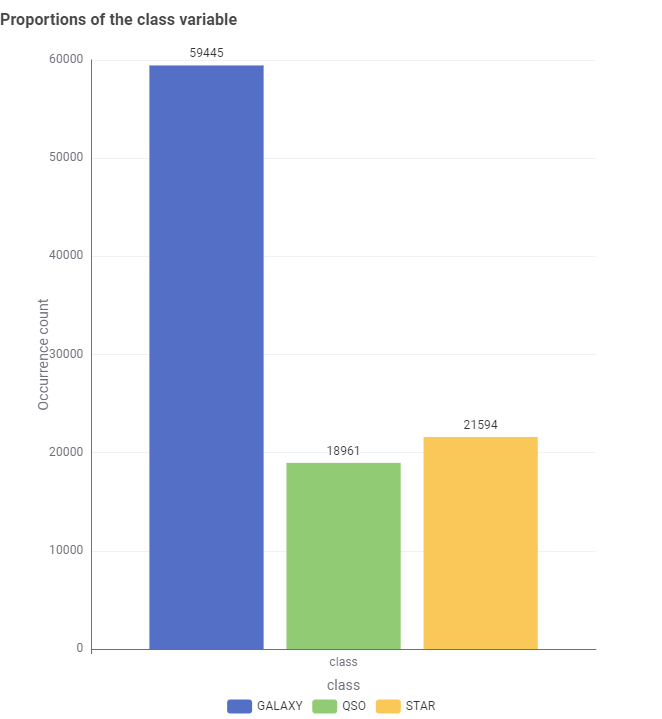
\includegraphics[width=1\columnwidth]{images/Bar Chart.png}
    \caption{Proportions of the unbalanced dataset.}
    \label{fig:classes}
\end{figure}
%Following, there are the number of observations for the class variable:
%\begin{itemize}
%    \item Galaxies: 59,445.
%    \item Quasars: 18,961.
%    \item Stars: 21,594.
%\end{itemize}

As we can see from Fig.~\ref{fig:classes}, quasars appeared less frequently compared to galaxies and stars, aligning with the expectation that quasars are rarer and further celestial objects.\\The dataset is \textit{unbalanced} with respect to the target variable. This needs to be taken into account and addressed, and it will be further analyzed.
%\vspace{0.5cm}
\section{Data Preparation}
In order to make the data more suitable for the classification task, some preprocessing steps have been applied, including dealing with outliers, checking for possible missing values, column filtering and normalizing the dataset.
%\bigskip
%\subsection{Outlier Detection, Missing Values, Column Filter, Normalizer}
\subsection{Preprocessing and Transformation}
After reading our dataset, we handled numeric \textit{outliers} by using the suited KNIME node, which identifies outliers using the \textit{Interquartile Range (IQR)}. 

After dealing with the outliers, a \textit{missing value} node is used to manage this issue, replacing missing integers and doubles with a median value and dropping rows with missing string values in a column. Even though no missing values were observed in the dataset, this handling is still performed to enable an eventual scalability.

Afterwards, the important features that were determined by Feature Importance process were retained to reduce noise and computations. The \texttt{spec-obj-ID} feature is also maintained: even though it seems to have less importance, it is actually a critical element for differentiating each class, as described in the Section~\ref{sec:ds_desc}. 

Then, we have applied Z-score normalization on the selected columns to scale our data such that the values are normally distributed. This ensured that no single feature affected the model disproportionally.
%Since our dataset is an unbalanced data set, meaning that some classes have objectively more values than the others, undersampling has been applied to the majority class in order to make the values more balanced. Equal Size Sampling node is used for this purpose. Normalizer node is used to transform the values into a consistent state. This ensured that no single feature affected the model disproportionally. SMOTE is also used throughout the design in order to produce synthetic values in order to further balance the dataset.
\subsection{Exploratory Data Analysis}
Exploratory data analysis methodologies are applied in order to visualize the data distributions and correlations, and improve understanding beforehand. 

We mainly produced a linear correlation matrix (as visible in Fig.~\ref{fig:corrmatrix}) between features, and it emerged that the features with the highest correlation values with \texttt{class} are \texttt{u}, \texttt{g} and \texttt{redshift}.
\vspace{-1.5cm}
\begin{figure}[H]
    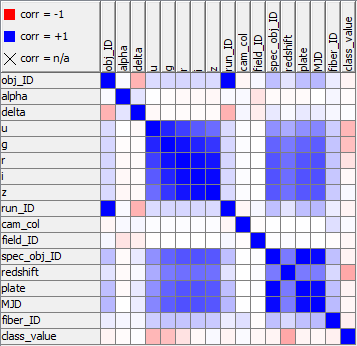
\includegraphics[width=0.9\columnwidth]{images/Correlation Matrix.png}
    \centering
    \caption{Feature correlation matrix.}
    \label{fig:corrmatrix}
\end{figure}
\vspace{-3cm}
The exploration of the relationship of \texttt{u} and \texttt{g} with other features displayed difficulties for determining the class of the observations. Despite this, we decided to further explore \texttt{redshift} against other features, and this led to the conclusion that \texttt{redshift} is the most significant feature to classify our records.
%\vspace{-0.3cm}
\subsection{Feature Importance}
Feature importance has been applied to detect the most important features and use them to reduce computations and noise, without losing relevant information. This has been implemented with Tree Ensemble, which learns an ensemble of decision trees, such as Random Forest variants. This method gave us an importance score for each feature, allowing us to understand their relative significance in the classification task.   
\begin{figure}[H]
    \centering
    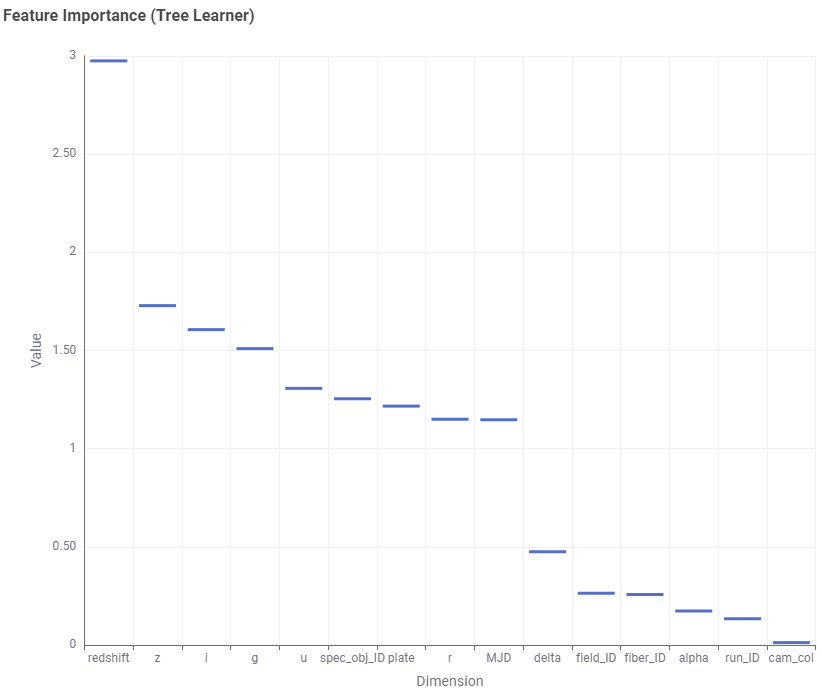
\includegraphics[width=1\columnwidth]{images/Feature Importance.png}
    \caption{Feature Importance based on Tree Learner.}
    \label{fig:fig2}
\end{figure}
We used every feature with a score value greater than 1, except for \texttt{MJD} and \texttt{plate}.\\We excluded these two because it turned out that they do not affect performance at all.
\section{Classification Models}
In this project, various classification techniques were used to identify the most suitable approach. Seven classifiers were applied throughout the Knime workflow, categorized into the following 4 groups:
%\bigskip
\begin{itemize}
    \item \textbf{Heuristic Models}: In this project, Decision Tree (J48), k-Nearest Neighbor (kNN), Random Forest and XGBoost (specific implementation of Gradient Boosting) are applied.
    \item \textbf{Regression based Models}: Logistic regression is used, which models a linear relationship between inputs and a categorical output, using a parametric conditional probability.
    \item \textbf{Separation Models}: Support Vector Machine (Weka's SMO implementation) and Multi-Layer Perceptron are used, which both partition the attributes' space.
    \item \textbf{Probabilistic Models}: Naive Bayes is applied, exploiting Bayes formula and computing posterior probability to classify records.
\end{itemize}

\subsection{Performance Measures}
To evaluate the performance of the models, a variety of measures were computed. These metrics provide a detailed evaluation of classification performance under different conditions. The measures applied are the following:
\begin{itemize}
    \item \textbf{Accuracy}: The number of correct predictions on the total number of predictions. It is calculated as follows:
    \[
    \text{Accuracy} = \frac{TP + TN}{TP + TN + FP + FN}
    \]
    Moreover, it measures the capability of the classification model to give reliable predictions on new records. However, the accuracy measure is not suitable for imbalanced datasets, as in our case. Therefore, the following measures are preferred.

    \item \textbf{Precision}: The fraction of correctly predicted positive records out of all positive predictions. It provides information on the ability of the model to minimize false positives.
    \[
    p = \frac{TP}{TP + FP}
    \]
    \item \textbf{Recall}: The fraction of actual positive records correctly identified by the model. It provides information on the ability of the model to minimize false negatives.
    \[
    r = \frac{TP}{TP + FN}
    \]
    
\end{itemize}

\begin{itemize}
    \item $F_1$ \textbf{measure}: Combines precision ($p$) and recall ($r$) into a single metric by calculating their harmonic mean:
    \[
    F_{measure} = \frac{2 \cdot r \cdot p}{r + p}
    \]
    \item \textbf{ROC and AUC}: The Receiver Operating Characteristic (ROC) curve plots the True Positive Rate (TPR) against the False Positive Rate (FPR) at various classification thresholds. The ROC curve depicts the performance of a classifier without regard to class distribution. Thus, it is useful for confronting different classification models, considering the Area Under the Curve (AUC) value. It ranges from 0 to 1 and measures the overall performance of the classifier. The closer it is to 1, the closer the classifier has TPR to 1 (ideal classifier).
        \begin{figure}[H]
            \centering
            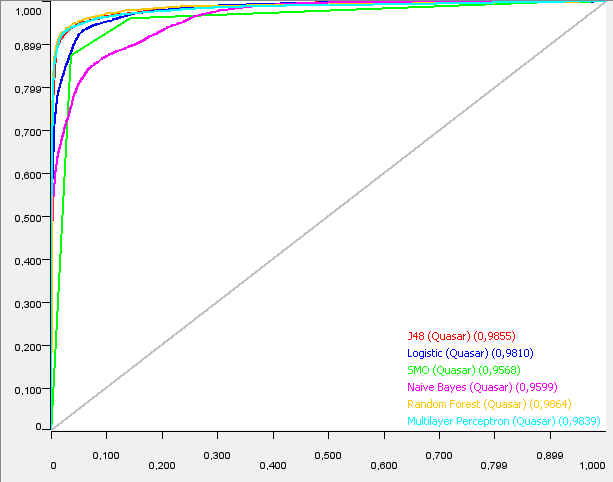
\includegraphics[width=0.9\columnwidth]{images/ROC Quasar MultiClass KFold.png}
            \caption{ROC of Quasar class (initially the least occurrent label) for balanced data from the MultiClassClassifier node.}
            \label{fig:roc_qso_multiclass_kfold}
        \end{figure}
\end{itemize}
\section{Classification and Results}
%\bigskip
This section presents and compares the results of the classification methods to determine the optimal model. Before evaluating them, the impact of class imbalance is examined by comparing models for balanced and imbalanced dataset. Additionally, the performance of Holdout and k-fold Cross-Validation is assessed for both the Classification with the specific learner nodes, and the Classification employing a metaclassifier node. 
To effectively handle multi-class datasets using native binary classifiers, the MultiClass Classifier node was employed~\cite{multiclasswiki}. It decomposes multi-class problems into multiple binary classification tasks, enabling a structured comparison between binary classification models and those adapted for multi-class scenarios.

The performance was evaluated using multiple measures, including Accuracy, F1-Measure, Recall, Precision, and AUC. The analysis aimed to compare the effectiveness of various classifiers using different approaches.
Furthermore, to facilitate a comprehensive analysis of model performance, the results obtained from different classification methods were combined, providing a clearer and more structured evaluation framework.

\subsection{Comparison with Imbalanced Dataset}
\subsubsection{Holdout}
The holdout method is a widely used validation technique for assessing the performance of classification models by dividing the dataset into training and testing subsets. The dataset was partitioned using an 80\%-20\% split, where 80\% of the data was allocated for training and 20\% for testing.
\subsubsection{k-folds Cross Validation}
K-fold Cross-Validation is a robust technique for evaluating the performance of classification models by partitioning the dataset into multiple subsets, ensuring a more reliable assessment of generalization error. In this study, a 5-fold cross-validation procedure was implemented for every model, dividing the dataset into five equal subsets. Each subset was used once as a test set while the remaining four subsets were used for training, allowing every data point to contribute to both training and testing. This process provides a more stable estimate of model performance. The cross-validation procedure was carried out using the X-Partitioner node.
\subsection{Comparison with Balanced Dataset}
\subsubsection{Equal Size Sampling}
As already mentioned, class imbalance is a critical issue in classification tasks, where an unequal distribution of class instances can lead to biased models that favour the majority class, thereby reducing the predictive performance for minority classes. Different techniques can be employed to correct class imbalance~\cite{imbalancedknime}, including downsampling the majority class, or oversampling the minority class through methods such as the \textit{Synthetic Minority Over-sampling Technique (SMOTE)}~\cite{imbalancedwiki}. For our case, \textit{Equal Size Sampling} was applied the node of the same name, which systematically removes instances from the dataset to ensure an equal distribution of classes within a nominal variable. By ensuring balanced class representation, classification models can achieve improved generalization error and more reliable performance across all categories.
\subsubsection{Holdout}
As before, the holdout method was also applied to the balanced dataset using an 80\%-20\% split. Balancing the dataset ensures that models do not favour the majority class, leading to a more representative evaluation of classification performance.
\subsubsection{k-folds Cross Validation}
The same considerations made in the corresponding section of the imbalanced case also apply here.
\subsection{Feature Selection}% Implemented Classification on Balanced Dataset}
Feature selection is a crucial step in classification, aiming to identify the most relevant variables while reducing redundancy and improving model efficiency. When applied to a balanced dataset, it ensures that the selected features are not biased towards the majority class, leading to more reliable predictions. 

To enhance analysis, both Filter approaches and Wrapper method were implemented, allowing a clearer assessment of feature selection and classification performance.
\subsubsection{Univariate Filter}
Univariate Filter was performed using the \textit{AttributeSelectedClassifier} node in KNIME. Using this method, attributes are selected before learning the classifier through an objective function. The \texttt{Ranker} search method was applied, evaluating each feature individually based on statistical criteria, such as \textit{Information Gain Ratio}, which evaluates the worth of an attribute by measuring the information gain with respect to the class. This approach ranks attributes selecting the top five most relevant features for classification. Univariate filtering is computationally efficient and straightforward, making it effective for reducing dimensionality. However, it does not take into account for relationships between attributes, which may result in the selection of redundant variables.
\subsubsection{Multivariate Filter}
Multivariate Filter was conducted with the same node but with the \texttt{BestFirst} search method. Unlike univariate approaches, this one evaluates feature subsets rather than individual attributes, allowing for the identification of the most informative combinations. This method explores different subsets by considering interactions between features, ensuring that selected attributes contribute unique information to the model. Although more computationally intensive, multivariate filters typically lead to improved classification performance by reducing redundancy and capturing complex relationships within the data. In this study, this solution selects only two features, compared to the 5 features selected by the univariate filter, but with similar performance.
\subsubsection{Wrapper}
In this project, the Wrapper method was employed for feature selection using the same node used for the Filter method, although configured with the \texttt{WrapperSubsetEval} evaluator. Wrappers assess the usefulness of feature subsets by evaluating their impact on a specific classifier's performance, effectively tailoring the feature selection process to the model in use. In our case, the evaluator conducts a 5-fold Cross-Validation to estimate the accuracy of the learning scheme for a set of attributes. This involves partitioning the dataset into five subsets, sequentially using each subset for testing while training on the remaining data. 

The wrapper method is significantly computationally intensive due to the iterative nature of the process. This approach is particularly advantageous when interactions between features significantly influence model performance. It is worth noting that kNN, MLP, and SMO models were excluded due to their high computational cost, which made the feature selection process using wrapper excessively time-consuming.
\subsection{Results}
The performance of the classification models was evaluated using multiple metrics, including Accuracy, F1-Measure, Recall, Precision, and Area Under the Curve (AUC). The analysis aimed to compare the effectiveness of various classifiers. 
As already discussed, Accuracy is less robust and informative when applied to imbalanced datasets, because it may yield misleading results due to the disproportionate class distribution. For this reason, other measures (such as F1-measure, Recall, Precision) are preferred for the evaluation of the imbalanced configuration. 
Therefore, the Accuracy and AUC values of the balanced dataset for the metaclassifier node are highlighted in this report. In fact, the tables below show the accuracy performance evaluation of the metaclassifier learner for the holdout and cross-validation methods. 
\begin{table}[H]
\centering
\label{tab:without_cv}
\begin{tabular}{|l|c|}
\hline
\textbf{Model} & \textbf{Accuracy} \\ \hline
Random Forest & 0.964 \\ \hline
Random Forest\_CV & 0.961 \\ \hline
Multilayer Perceptron & 0.962 \\ \hline
Multilayer Perceptron\_CV & 0.957 \\ \hline
J48 & 0.960 \\ \hline
J48\_CV & 0.956 \\ \hline
Logistic Regression & 0.936 \\ \hline
Logistic Regression\_CV & 0.934 \\ \hline
Naïve Bayes& 0.884 \\ \hline
Naïve Bayes\_CV & 0.886 \\ \hline
SMO & 0.839 \\ \hline
SMO\_CV & 0.839 \\ \hline
\end{tabular}
\caption{Model Accuracy for MultiClassClassifier node (with Holdout and CV=Cross-Validation)}
\end{table}

The analysis reveals that the top-performing models for both methodologies are consistent, with Random Forest, Multilayer Perceptron, and J48 showing nearly identical performance metrics. 

The tables below present the AUC values achieved by each model, categorized by class value and methodology (holdout and CV). Notably, Random Forest demonstrates the highest AUC values across the evaluated conditions. 

\begin{table}[H]
\centering
\resizebox{\linewidth}{!}{
\begin{tabular}{|l|c|}
\hline
\textbf{Classifier} & \textbf{Area Under Curve} \\
\hline
\textbf{Random Forest (Star)\_CV} & \textbf{1} \\
\textbf{Random Forest (Star)} & \textbf{1} \\
SMO (Star)\_CV & 0.988 \\
SMO (Star) & 0.99 \\
Naïve Bayes (Star)\_CV & 0.998 \\
Naïve Bayes (Star) & 0.998 \\
Multilayer Perceptron (Star)\_CV & 0.998 \\
Multilayer Perceptron (Star) & 0.999 \\
Logistic Regression (Star)\_CV & 0.998 \\
Logistic Regression (Star) & 0.999 \\
J48 (Star)\_CV & 0.998 \\
J48 (Star) & 0.999 \\
\hline
\end{tabular}
}
\caption{Area Under Curve for Star class (MultiClassClassifier node)}
\label{tab:star_auc}
\end{table}

% CHECK:
% I have fixed the output in theory @Selin @Fra
% Now I'm not checking, but I think we haven't done
% MLP at this step, I remember I left it only in Meta MultiClass


\begin{table}[H]
\centering
\resizebox{\linewidth}{!}{ % Automatically resize to fit width
\begin{tabular}{|l|c|}
\hline
\textbf{Classifier} & \textbf{Area Under Curve} \\
\hline
\textbf{Random Forest (Galaxy)\_CV} & \textbf{0.987} \\
\textbf{Random Forest (Galaxy)} & \textbf{0.988} \\
Multilayer Perceptron (Galaxy)\_CV & 0.981 \\
Multilayer Perceptron (Galaxy) & 0.985 \\
J48 (Galaxy)\_CV & 0.979 \\
J48 (Galaxy) & 0.982 \\
Logistic Regression (Galaxy)\_CV & 0.947 \\
Logistic Regression (Galaxy) & 0.952 \\
Naive Bayes (Galaxy)\_CV & 0.923 \\
Naive Bayes (Galaxy) & 0.921 \\
SMO (Galaxy)\_CV & 0.894 \\
SMO (Galaxy) & 0.899 \\
\hline
\end{tabular}
}
\caption{Area Under Curve for Galaxy class (MultiClassClassifier node)}
\label{tab:galaxy_auc}
\end{table}

\begin{table}[H]
\centering
\resizebox{\linewidth}{!}{
\begin{tabular}{|l|c|}
\hline
\textbf{Classifier} & \textbf{Area Under Curve} \\
\hline
\textbf{Random Forest (Quasar)\_CV} & \textbf{0.986} \\
\textbf{Random Forest (Quasar)} & \textbf{0.988} \\
Multilayer Perceptron (Quasar)\_CV & 0.984 \\
Multilayer Perceptron (Quasar) & 0.986 \\
J48 (Quasar)\_CV & 0.985 \\
J48 (Quasar) & 0.988 \\
Logistic Regression (Quasar)\_CV & 0.981 \\
Logistic Regression (Quasar) & 0.983 \\
Naive Bayes (Quasar)\_CV & 0.96 \\
Naive Bayes (Quasar) & 0.96 \\
SMO (Quasar)\_CV & 0.957 \\
SMO (Quasar) & 0.959 \\
\hline
\end{tabular}
}
\caption{Area Under Curve for Quasar class (MultiClassClassifier node)}
\label{tab:quasar_auc}
\end{table}

Moreover, the table below shows the Accuracy values for the specific Learner nodes which perform also XGBoost and kNN, in addition to Random Forest and the other classifiers that have already been evaluated before. In this case, we observe a high accuracy for XGBoost, both for holdout and CV, comparable to the Random Forest. 
\begin{table}[H]
\centering
\label{tab:other_classifiers_specific}
\begin{tabular}{|l|c|}
\hline
\textbf{Model} & \textbf{Accuracy} \\ \hline
\textbf{XGBoost} & \textbf{0.962} \\ \hline
\textbf{XGBoost\_CV} & \textbf{0.961} \\ \hline
\textbf{Random Forest} & \textbf{0.962} \\ \hline
\textbf{Random Forest\_CV} & \textbf{0.959} \\ \hline
kNN & 0.95 \\ \hline
kNN\_CV & 0.945 \\ \hline
\end{tabular}
\caption{Model Accuracy for specific Learner nodes}
\end{table}
%\vspace{0.3cm}
\section{Conclusions}
%\bigskip
%After implementing preprocessing and visualization strategies before carefully analyzing our data,

The objective of this project consisted in determining one or more multiclass classification models that allow to accurately predict the category of astronomical objects. 
It emerged that the important aspects are the redshift and the photometric filters. From these initial discoveries, we then performed the effective classification task and compared the results using different methods, like comparing imbalanced and balanced datasets, techniques such as k-folds Cross-Validation and hold-out. Finally, we also applied filter and wrapper approaches for feature selection process in order to retain the most crucial attributes and reduce noise and computational load.

Then, we evaluated the performance of the following models with hold-out and k-fold Cross-Validation: XGBoost, Random Forest, kNN, J48 (Decision Tree), Logistic Regression, Naive Bayes, Multi-Layer Perceptron, SMO (Support Vector Machine). Analyzing all these classifiers for multiclass classification task, XGBoost and Random Forest turned out to be the optimal solution for specific learners approach, while Random Forest emerged to be the best one also for metaclassifier.\\
To be more precise, both XGBoost and Random Forest achieve approximately an accuracy of 96\%.
%Generally, the classification models involved are among the ones typically suited for multiclass classification problems, although Support Vector Machine and Logistic Regression do not support multi-class classification by default.
Regarding the class imbalance problem, Equal Size Sampling was discovered to be the best approach, considering performances and computational time, also avoiding favouring the majority class, as it would happen with class imbalance.

Finally, feature selection played a pivotal role in enhancing classification performance by identifying the most relevant variables among the 15 columns available - removing earlier \texttt{obj\_id} and \texttt{run\_id} from the original 17 - while also reducing redundancy. Both Filter and Wrapper approaches were implemented, each offering distinct advantages. The Univariate Filter, utilizing the Ranker method and Information Gain Ratio, efficiently selected 5 features, but this method doesn't take into account inter-attribute relationships. In contrast, the Multivariate Filter with CFS and BestFirst search method identified only 2 features while maintaining similar performance, demonstrating the benefits of evaluating feature subsets for capturing complex relationships. Then, the Wrapper method, though computationally intensive, provided tailored feature selection through 5-fold Cross-Validation. Despite its potential for higher F-measure and accuracy, models such as kNN, XGBoost, MLP, and SMO were excluded due to excessive computational demands. It emerged that with this method, J48 and Random Forest achieve the highest values for F-measure and accuracy, respectively selecting 4 and 6 features. However, we have to keep in mind of the trade-off between performance and computational efficiency for feature selection strategies.

From this study, it is clear that the chosen stellar dataset is natively effective and optimized for the classification of stars, galaxies and quasars. Therefore, it allows getting high performance and clear understanding without requiring additional features and overall pre-processing. 

%\vspace{0.4cm}
%\bibliographystyle{plain}
%\bibliography{references}
\printbibliography
\end{multicols}
\end{document}
